\documentclass{article}
\usepackage[T1]{fontenc}
\usepackage{lmodern}
\usepackage{graphicx}
\usepackage{amsmath,amssymb}
\usepackage[a4paper,margin=2cm]{geometry}
\usepackage[absolute,overlay]{textpos}
\setlength{\TPHorizModule}{1mm}
\setlength{\TPVertModule}{1mm}
\usepackage[indonesian]{babel}
\usepackage{hyperref}
\setlength{\emergencystretch}{2em}
% unit: Halaman 3

\begin{document}

% === Halaman 3 (python/native) ===

• FYI, Alice dan Bob di dalam dunia nyata bisa berupa 


- Alice dan Bob adalah manusia dalam arti sesungguhnya


- manusia dengan mesin (misalnya mesin penjawab telepon)

             - mesin dengan mesin (misalnya komputer client dengan komputer server)


- web browser dengan sistem server di dalam jaringan komputer


- online banking client/server


- DNS server, router, mesin penjawab telepon, dsb

3

% deskripsi: gambar native xref 30
\noindent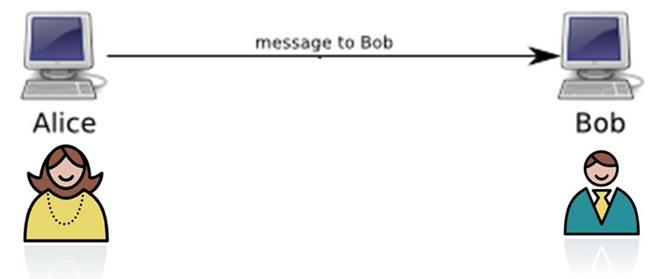
\includegraphics[width=0.85\textwidth]{../../images/python/page_003_img_01.jpeg}

\end{document}
